\documentclass[a4paper, 12pt]{article}
% packages
\usepackage{amssymb}
\usepackage[fleqn]{mathtools}
\usepackage{tikz}
\usepackage{enumerate}
\usepackage{bussproofs}
\usepackage{xcolor}
\usepackage[margin=1.3cm]{geometry}
\usepackage{logicproof}
\usepackage{diagbox}

% augmented matrix
\makeatletter
\renewcommand*\env@matrix[1][*\c@MaxMatrixCols c]{%
\hskip -\arraycolsep
\let\@ifnextchar\new@ifnextchar
\array{#1}}
\makeatother

% ceiling / floor
\DeclarePairedDelimiter{\ceil}{\lceil}{\rceil}
\DeclarePairedDelimiter{\floor}{\lfloor}{\rfloor}

% custom commands
\newcommand{\indefint}[2]{\int #1 \, \mathrm{d}#2}
\newcommand{\defint}[4]{\int_#1^#2 #3 \, \mathrm{d}#4}
\newcommand{\dif}[2]{\frac{\mathrm{d}#1}{\mathrm{d}#2}}
\newcommand{\limit}[2]{\displaystyle{\lim_{#1 \to #2}}}
\newcommand{\summation}[3]{\sum\limits_{#1}^#2 #3}
\newcommand{\intbracket}[3]{\left[#3\right]_#1^#2}

\newcommand{\powerset}[0]{\wp}
\renewcommand{\emptyset}[0]{\varnothing}

\newcommand{\unaryproof}[2]{\AxiomC{#1} \UnaryInfC{#2} \DisplayProof}
\newcommand{\binaryproof}[3]{\AxiomC{#1} \AxiomC{#2} \BinaryInfC{#3} \DisplayProof}

% no indent
\setlength\parindent{0pt}

% reasoning proofs
\newcommand{\proofline}[3]{(#1)\ & #2 & \text{#3} \\}
\allowdisplaybreaks

% actual document
\begin{document}
    \section*{CO112 - Hardware}
        \subsection*{Prelude}
            The content discussed here is part of CO112 - Hardware (Computing MEng); taught by Bernhard Kainz, and Bjoern Schuller, in Imperial College London during the academic year 2018/19. The notes are written for my personal use, and have no guarantee of being correct (although I hope it is, for my own sake). This should be used in conjunction with the notes, and lecture slides.
        \subsection*{Notes - Lecture 1}
            This section will be covered in less detail, as we've gone through. However, we will need to change the notation we use in this course from the one used in logic, from using $\land$ to $\cdot$, $\lor$ to $+$, and from $\neg$ to $^\prime$.
            \begin{center}
                \begin{tabular}{cc|c|c|c}
                    $A$ & $B$ & $A \cdot B$ (AND) & $A + B$ (OR) & $A^\prime$ (NOT) \\
                    \hline
                    0 & 0 & 0 & 0 & 1 \\
                    0 & 1 & 0 & 1 & 1 \\
                    1 & 0 & 0 & 1 & 0 \\
                    1 & 1 & 1 & 1 & 0
                \end{tabular}
            \end{center}
        \subsection*{Panopto - Lecture 14}
            Putting together a manual processor; generally the block diagram takes in a sequence of binary numbers, one sequence for data, and another for instructions. This will result in a binary number. Our design is based on the von Neumann architecture, which divides the processor into arithmetic units and registers, with a shared stream for data, and intstructions. Our model will be based on 8 bits.
            \medskip

            Our example action is to find the average of two numbers, $A$, and $B$, such that $R = \frac{A + B}{2}$. Since we are dealing with 8 bits, $A + B < 256$.
            \begin{enumerate}[1.]
                \itemsep0em
                \item The first number is set up in input lines, and stored in register (A)
                \item The same is done for the second number, and stored in register (B)
                \item The arithmetic circuits are set to register (A) to (B).
                \item The resulting sum is put into (A)
                \item The shift circuits shift (A) one bit to the right, which is integer division by 2
                \item Result is loaded into (Res).
            \end{enumerate}
            In order to do this, we need a number of components;
            \begin{itemize}
                \item Registers
                    \begin{itemize}
                        \item store data (A), and (B)
                        \item store result (Res)
                        \item one bit for carry (C)
                        \item store instruction (IR)
                    \end{itemize}
                \item Arithmetic circuits
                    \begin{itemize}
                        \item 8-bit adder
                        \item 8-bit shifter
                    \end{itemize}
            \end{itemize}
            Note in the figure below, that the 8 means it is an 8-bit line.

            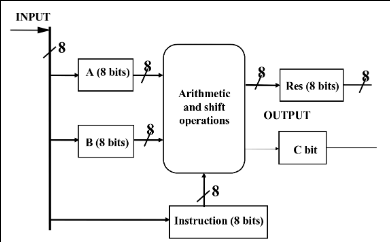
\includegraphics[width=0.5\linewidth]{2019-04-08-15-00-51.png}
        \subsection*{Notes - Lecture 14}


\end{document}
